\section{PROPOSED APPROACH}
\label{sec:proposed_approach}

\subsection{Data Sources and Collection}
Data was collected from three main sources: surveillance radar data for civil flights landing in São Paulo/Guarulhos International Airport (ICAO: SBGR) was provided by Operational Data Integrator (ODIN) from Brazilian Airspace Control Institute (ICEA), flight-condition fuel usage for aircraft was extracted from Base of Aircraft Data (BADA) online API \cite{bada_a320} and climate data, including ceiling and visibility, was downloaded from Iowa State University API.

\subsubsection{ODIN Surveillance Radar Data}
ICEA's ODIN contains operational registries for air traffic all around Brazilian territory, including data from five radar arrays around Brazil: \textit{Amazônico} (located in north), \textit{Brasilia} (center-west), \textit{Recife} (northeast), \textit{Curitiba} (south) and \textit{Atlântico} (oceanic portion). They provide information for latitude, longitude, speed relative to sound, flight level, call sign registration and datetime for registry.

Also, ODIN provides previously calculated KPI08 data \cite{mca10022}, including departure airport, landing airport, call sign, weight class and type for aircraft, landing runway, datetime for entering in Terminal Maneuvering Area (TMA) and KPI08 metric itself \cite{doc9750}. Table \ref{tab:odin_dict} summarizes the specific fields from the ODIN surveillance and KPI08 datasets utilized in this work.

\begin{table}[htbp]
\caption{Data Dictionary for ODIN Surveillance Radar Data}
\label{tab:odin_dict}
\centering
\begin{tabular}{m{0.28\columnwidth} m{0.16\columnwidth} m{0.44\columnwidth}}
\hline
\textbf{Field} & \textbf{Type} & \textbf{Description} \\
\hline
\texttt{call\_sign} & String & Aircraft call sign registration \\
\texttt{adep} & String & Departure airport (ICAO code) \\
\texttt{ades} & String & Landing airport (ICAO code) \\
\texttt{aircraft\_type} & String & Aircraft model (e.g., A320) \\
\texttt{weight\_class} & String & Aircraft weight class (e.g., M, H) \\
\texttt{landing\_runway} & String & Validated landing runway (e.g., 09R) \\
\texttt{tma\_entry\_time} & Datetime & Datetime for entering the TMA \\
\texttt{kpi08} & Float & Calculated KPI08 metric (seconds) \\
\texttt{latitude} & Float & Aircraft latitude position \\
\texttt{longitude} & Float & Aircraft longitude position \\
\texttt{flight\_level} & Integer & Current flight level in hundreds of feet (e.g. 30) \\
\texttt{mach} & Float & Speed relative to sound (Mach) \\
\texttt{timestamp} & Datetime & Radar registry datetime \\
\hline
\end{tabular}
\end{table}

\subsubsection{BADA Efficiency Chart}
The aircraft efficiency map was computed using the Base of Aircraft Data (BADA) model \cite{bada_a320}, specifically BADA3, which accounts for, among other factors, the aircraft type and flight level in estimating instantaneous fuel consumption. The interface between the model and the study requirements was implemented through the \texttt{pyBADA} support library in Python \cite{pybada}. Table \ref{tab:bada_dict} presents the data dictionary for the BADA performance parameters extracted for our methodology.

\begin{table}[htbp]
\caption{Data Dictionary for BADA Efficiency Chart}
\label{tab:bada_dict}
\centering
\begin{tabular}{m{0.28\columnwidth} m{0.16\columnwidth} m{0.44\columnwidth}}
\hline
\textbf{Field} & \textbf{Type} & \textbf{Description} \\
\hline
\texttt{aircraft} & String & Aircraft model identifier (e.g., A320) \\
\texttt{tas\_ms} & Float & True Airspeed in meters per second \\
\texttt{fl} & Integer & Flight Level in hundreds of feet (e.g., 30) \\
\texttt{fuel\_flow\_kg\_s} & Float & Instantaneous fuel flow in kg/s \\
\hline
\end{tabular}
\end{table}

\subsubsection{Iowa State University Climate Data}
Iowa State University provides a public API for daily airport weather observations from around the world. In this article, studies will be focused on SBGR and will include both visibility and ceiling from observation radar. The specific fields retained from this dataset are described in Table \ref{tab:climate_dict}.

\begin{table}[htbp]
\caption{Data Dictionary for Iowa State University Climate Data}
\label{tab:climate_dict}
\centering
\begin{tabular}{m{0.28\columnwidth} m{0.16\columnwidth} m{0.44\columnwidth}}
\hline
\textbf{Field} & \textbf{Type} & \textbf{Description} \\
\hline
\texttt{valid} & Datetime & Observation timestamp (e.g., 2025-01-01 15:00) \\
\texttt{station} & String & Weather station ICAO code (e.g., SBSP) \\
\texttt{vsby} & Float & Visibility measurement (in miles) \\
\texttt{ceiling\_ft} & Float & Cloud ceiling height (in feet) \\
\hline
\end{tabular}
\end{table}

\subsection{Data Preparation and Feature Engineering}
The data for this paper were organized with possible scalability in mind. The source of the dataset is the Operational Data Integrator (ODIN) PostgreSQL database maintained by Brazilian Airspace Control Institute (ICEA); the records collected range from January 1 to December 31, 2025. Extraction was performed using Python scripts that produced Parquet files optimized for analytical workloads and stored locally. Subsequent data transformation employed DuckDB as the query engine, with transformations orchestrated through data build tool (dbt), forming a Medallion Architecture data pipeline \cite{databricks_medallion, saha_dataeng}. The resulting datasets were again exported as Parquet files for downstream analysis in Python. The stack used for this work is schematized on Figure \ref{fig:odin-etl-simplified}.

\begin{figure}[htbp]
    \centering
    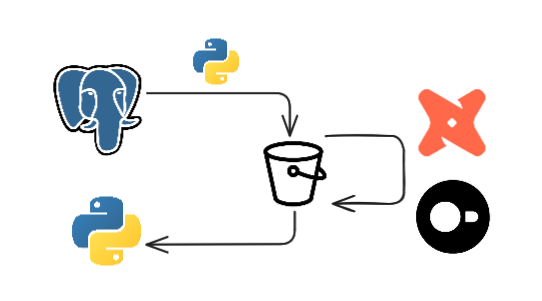
\includegraphics[width=1\linewidth]{images/odin-etl-simplified.png}
    \caption{Simplified schematics for the stack used in this work.}
    \label{fig:odin-etl-simplified}
\end{figure}

To enhance the analytical value of the flight data, a series of feature engineering transformations were applied using DuckDB and subsequently orchestrated and documented through dbt. We focused on creating features that better represented flight behavior, airspace congestion, and operational context.

The data transformations were structured across multiple SQL models to progressively build the final dataset:

\begin{itemize}
    \item \textbf{Trajectory Tracking and Elapsed Time:} The radar trajectory points were bounded between the time the aircraft crossed the TMA cylinder (\textit{c\_time}) and the actual landing time (\textit{aldt}). For each flight level (FL) recorded, the time difference between consecutive radar pings was calculated to establish the \textit{elapsed} time spent at each altitude.
    
    \item \textbf{Fuel Consumption Estimation:} The \textit{elapsed} time per flight level was multiplied by the aircraft's specific average fuel flow rate (kg/s) obtained from the BADA performance tables \cite{bada_a320, pybada}. The sum of these values across all flight levels yielded the total fuel consumption in the terminal area (\textit{consumption\_kg}).
    
    \item \textbf{Airspace Congestion Tracking:} To represent the dynamic traffic density, an event-based running sum was implemented. Every \textit{c\_time} was treated as an entry (+1) and every \textit{aldt} as an exit (-1). Using SQL window functions over the chronological timeline, we calculated the exact number of aircraft present in the TMA at any given moment (\textit{nr\_aircraft\_in\_tma}).
    
    \item \textbf{Rolling Predictive Metrics:} A moving average for the time spent in the TMA (\textit{transit\_tma\_predicted}) was created to mimic the expected transit time given recent conditions. This was calculated over a 1-hour rolling window preceding the flight, partitioned by the validated runway (\textit{drwy\_validado}) and the entry sector (\textit{setor}).
    
    \item \textbf{Baseline Efficiency and Target Variable:} To define a standard for efficient operations, we calculated the 20th percentile of fuel consumption (\textit{consumption\_20p}) partitioned by departure airport (\textit{adep}), aircraft type, and landing runway. Finally, the main target variable for this study, \textit{kpi16}, was computed as the difference between the actual fuel consumption (\textit{consumption\_kg}) and this 20th percentile baseline.
    
    \item \textbf{Temporal and Environmental Variables:} Datetime fields were decomposed into specific categories (\textit{day}, \textit{month}, \textit{hour}, and \textit{day of week}) to capture seasonal and daily patterns. Additionally, weather information from the METAR database (Iowa State University public API) was joined by the hour, incorporating horizontal visibility and cloud ceiling to assess their impact on flight holding and routing.
\end{itemize}

These transformations—ranging from chronological event tracking to percentile-based baselining—were carefully designed to expose underlying trends, airspace bottlenecks, and correlations within the flight data, paving the way for sophisticated machine learning investigations. Furthermore, adopting structured data modeling approaches (e.g., Medallion architecture) ensures scalability when applying these pipelines to massive Apache Spark or distributed SQL environments \cite{databricks_medallion, saha_dataeng}.

After the data transformation process, the variables can be classified into five main categories based on their purpose:
\begin{itemize}
    \item \textbf{Identification and temporal:} Unique flight identifier ($id$), date ($date$), day of the month ($day$), month ($month$), hour ($hour$), and day of the week ($dow$).
    \item \textbf{Operational:} Departure airport ($adep$), aircraft type ($aircraft$), validated landing runway ($drwy\_validado$), and TMA entry sector ($setor$).
    \item \textbf{Traffic and flight time:} Total transit time in TMA ($transit\_tma$), additional transit time ($kpi08$), number of aircraft in TMA ($nr\_aircraft\_in\_tma$), and predicted average transit time ($transit\_tma\_predicted$).
    \item \textbf{Meteorological:} Horizontal visibility ($visibility$) and cloud ceiling ($ceiling$).
    \item \textbf{Fuel consumption:} Total consumption in TMA ($consumption\_kg$), 20th percentile reference consumption ($consumption\_20p$), and additional consumption ($kpi16$).
\end{itemize}

\subsection{Exploratory Data Analysis}
The final dataset comprises 64,119 flight records representing landing operations at Guarulhos International Airport (SBGR) collected between January and December 2025. The dataset includes temporal, operational, traffic, meteorological, and fuel-consumption-related variables. An exploratory data analysis (EDA) was conducted to investigate the distribution of KPI16 and its relationship with the explanatory variables, as well as identify relevant patterns and highlight relationships that might influence the additional fuel consumption (KPI16) in the terminal area.

The distribution of $kpi16$ presents elongated tails, as shown in Figure \ref{fig:kpi16-distribution}, indicating the presence of observations with significantly high additional consumption. Such cases may be associated with adverse operational conditions, such as airspace congestion, unfavorable weather, or prolonged holding procedures. Outlier analysis was handled conservatively, maintaining observations between the 1st and 99th percentiles to preserve extreme events that represent actual operational behavior within the system.

\begin{figure}[htbp]
    \centering
    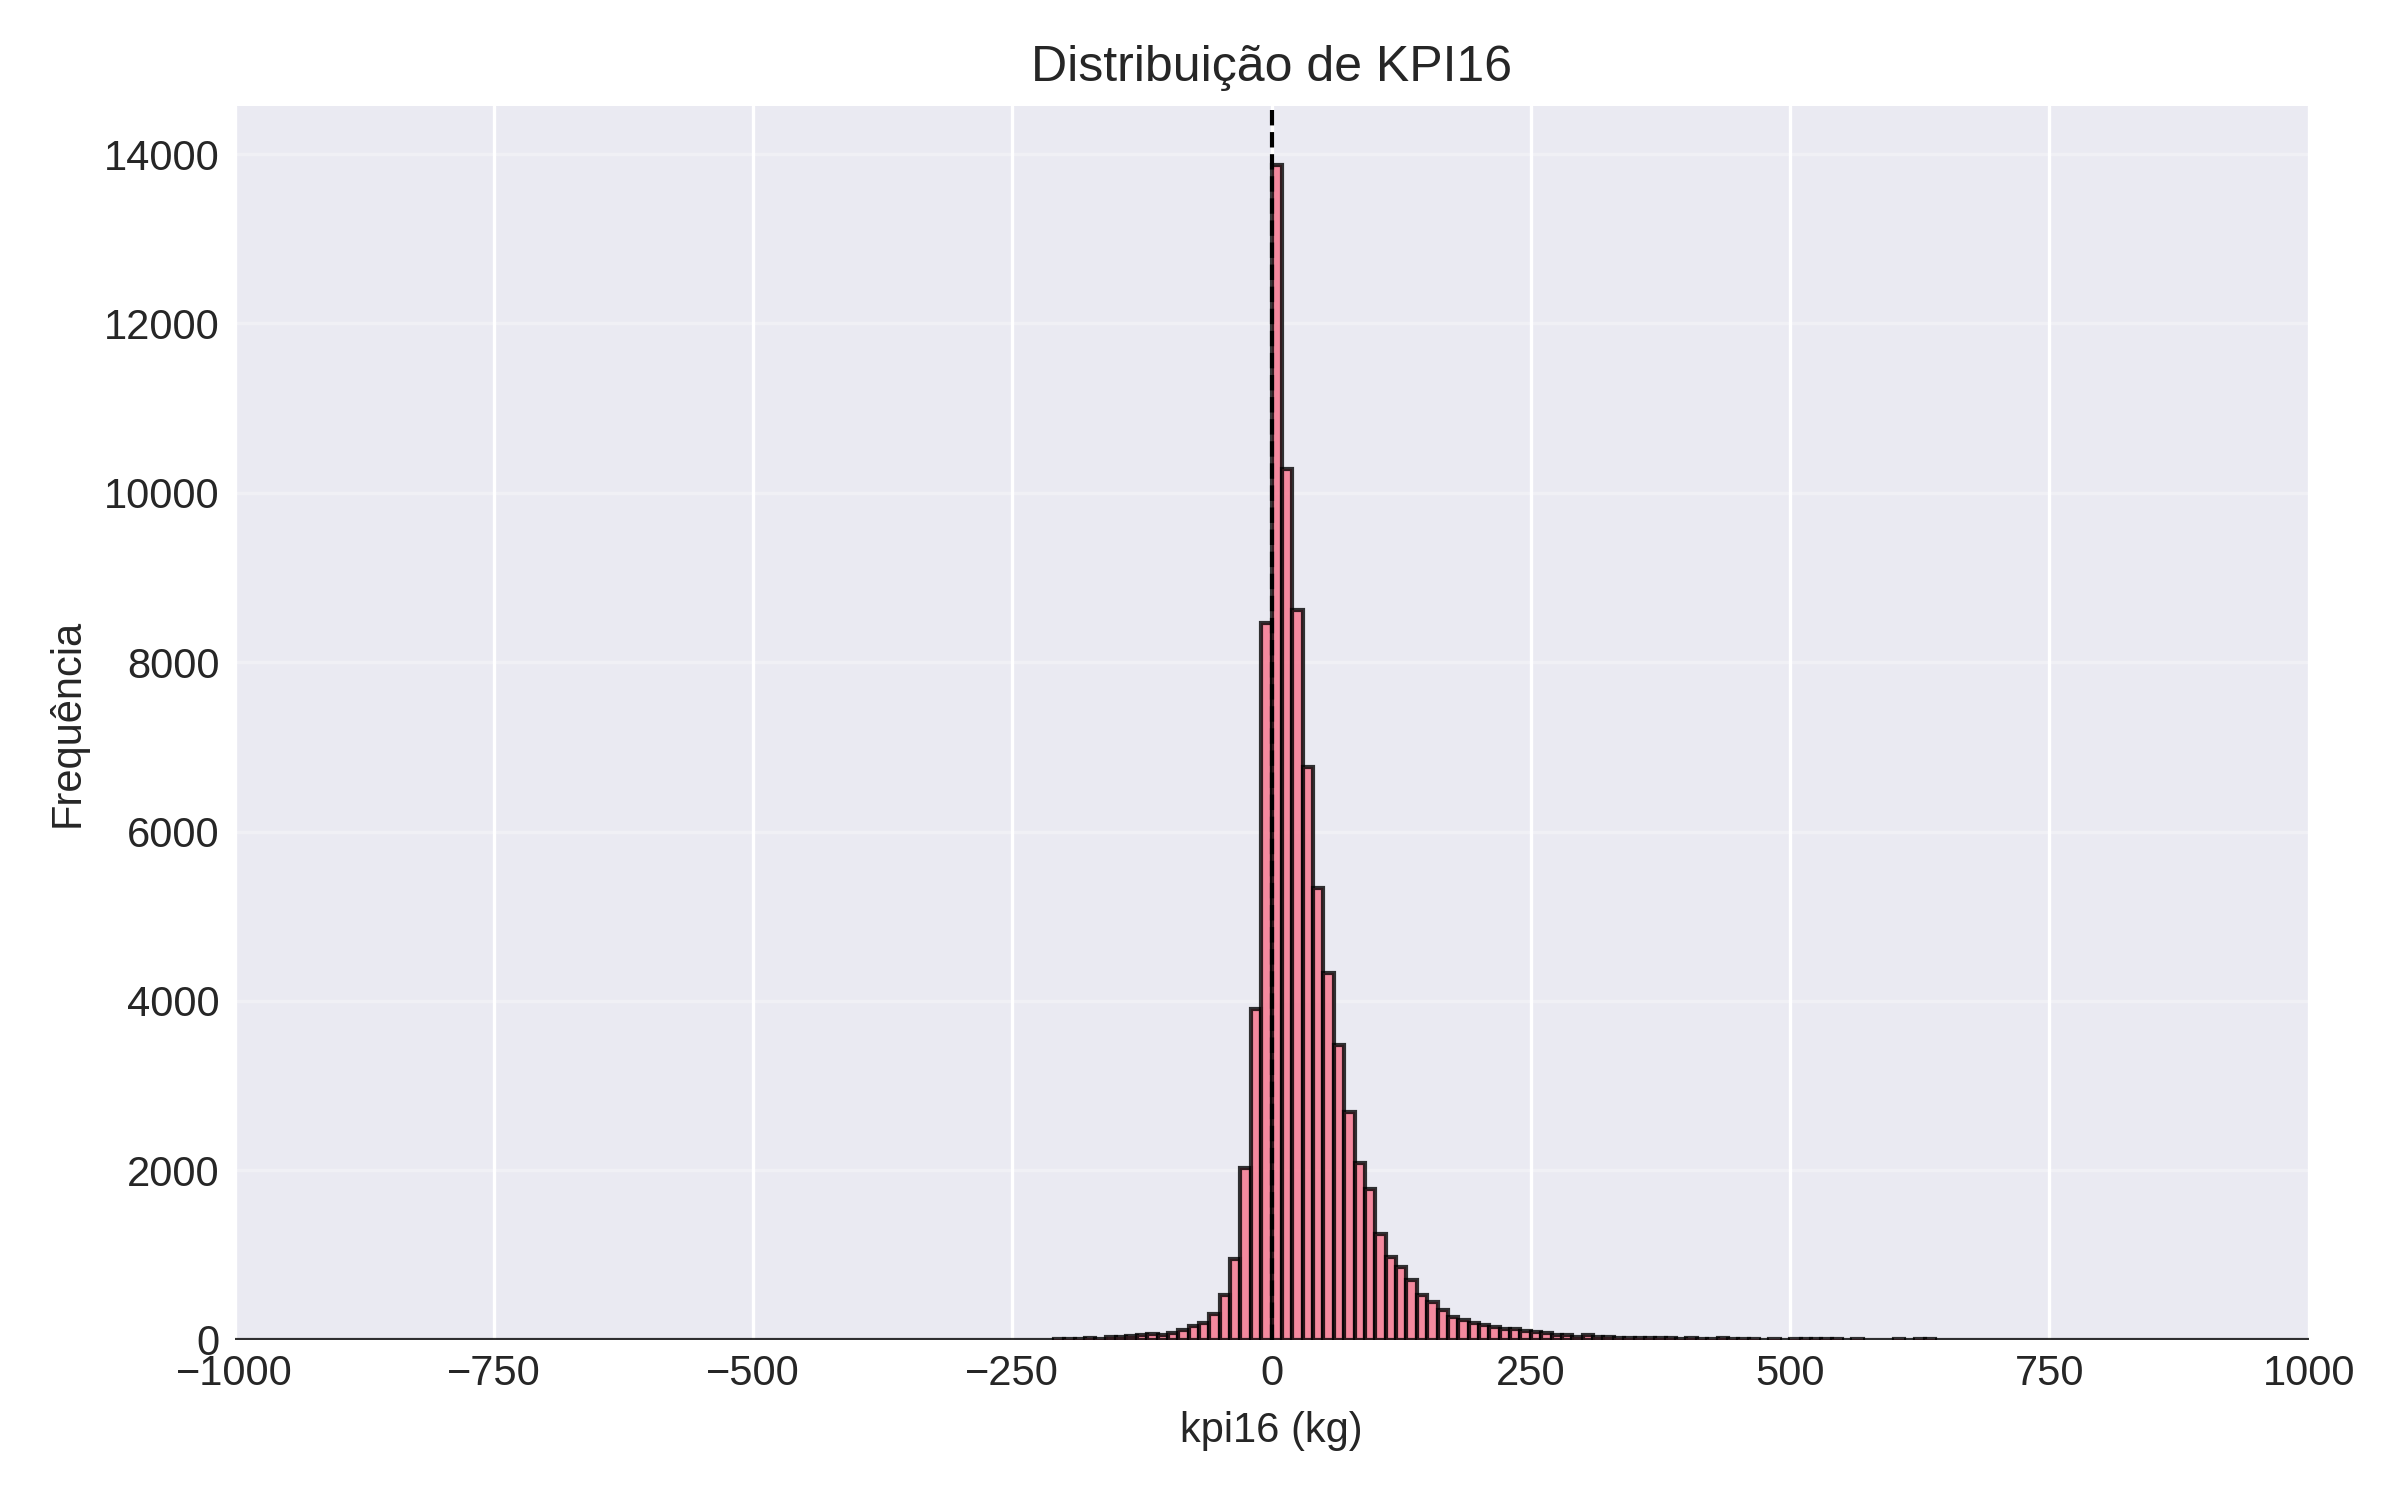
\includegraphics[width=1\linewidth]{images/kpi16-distribution.png}
    \caption{Distribution of the target variable $kpi16$ (Additional Fuel Consumption).}
    \label{fig:kpi16-distribution}
\end{figure}

\subsubsection{Additional Fuel Consumption by Departure Airport}
The departure airport (ADEP) plays a critical role in shaping the flight profile, cruise altitude, and approach procedure into the destination TMA. Figure \ref{fig:adep-kpi16} highlights the average additional fuel consumption (KPI16) for the 15 most frequent ADEPs. Notably, flights originating from Afonso Pena International Airport (SBCT) in Curitiba and Hercílio Luz International Airport (SBFL) in Florianópolis present the highest average penalties. This pattern suggests that these airports may share approach-related challenges, possibly associated with their geographical proximity and common entry routing into the Guarulhos TMA.

\begin{figure}[htbp]
    \centering
    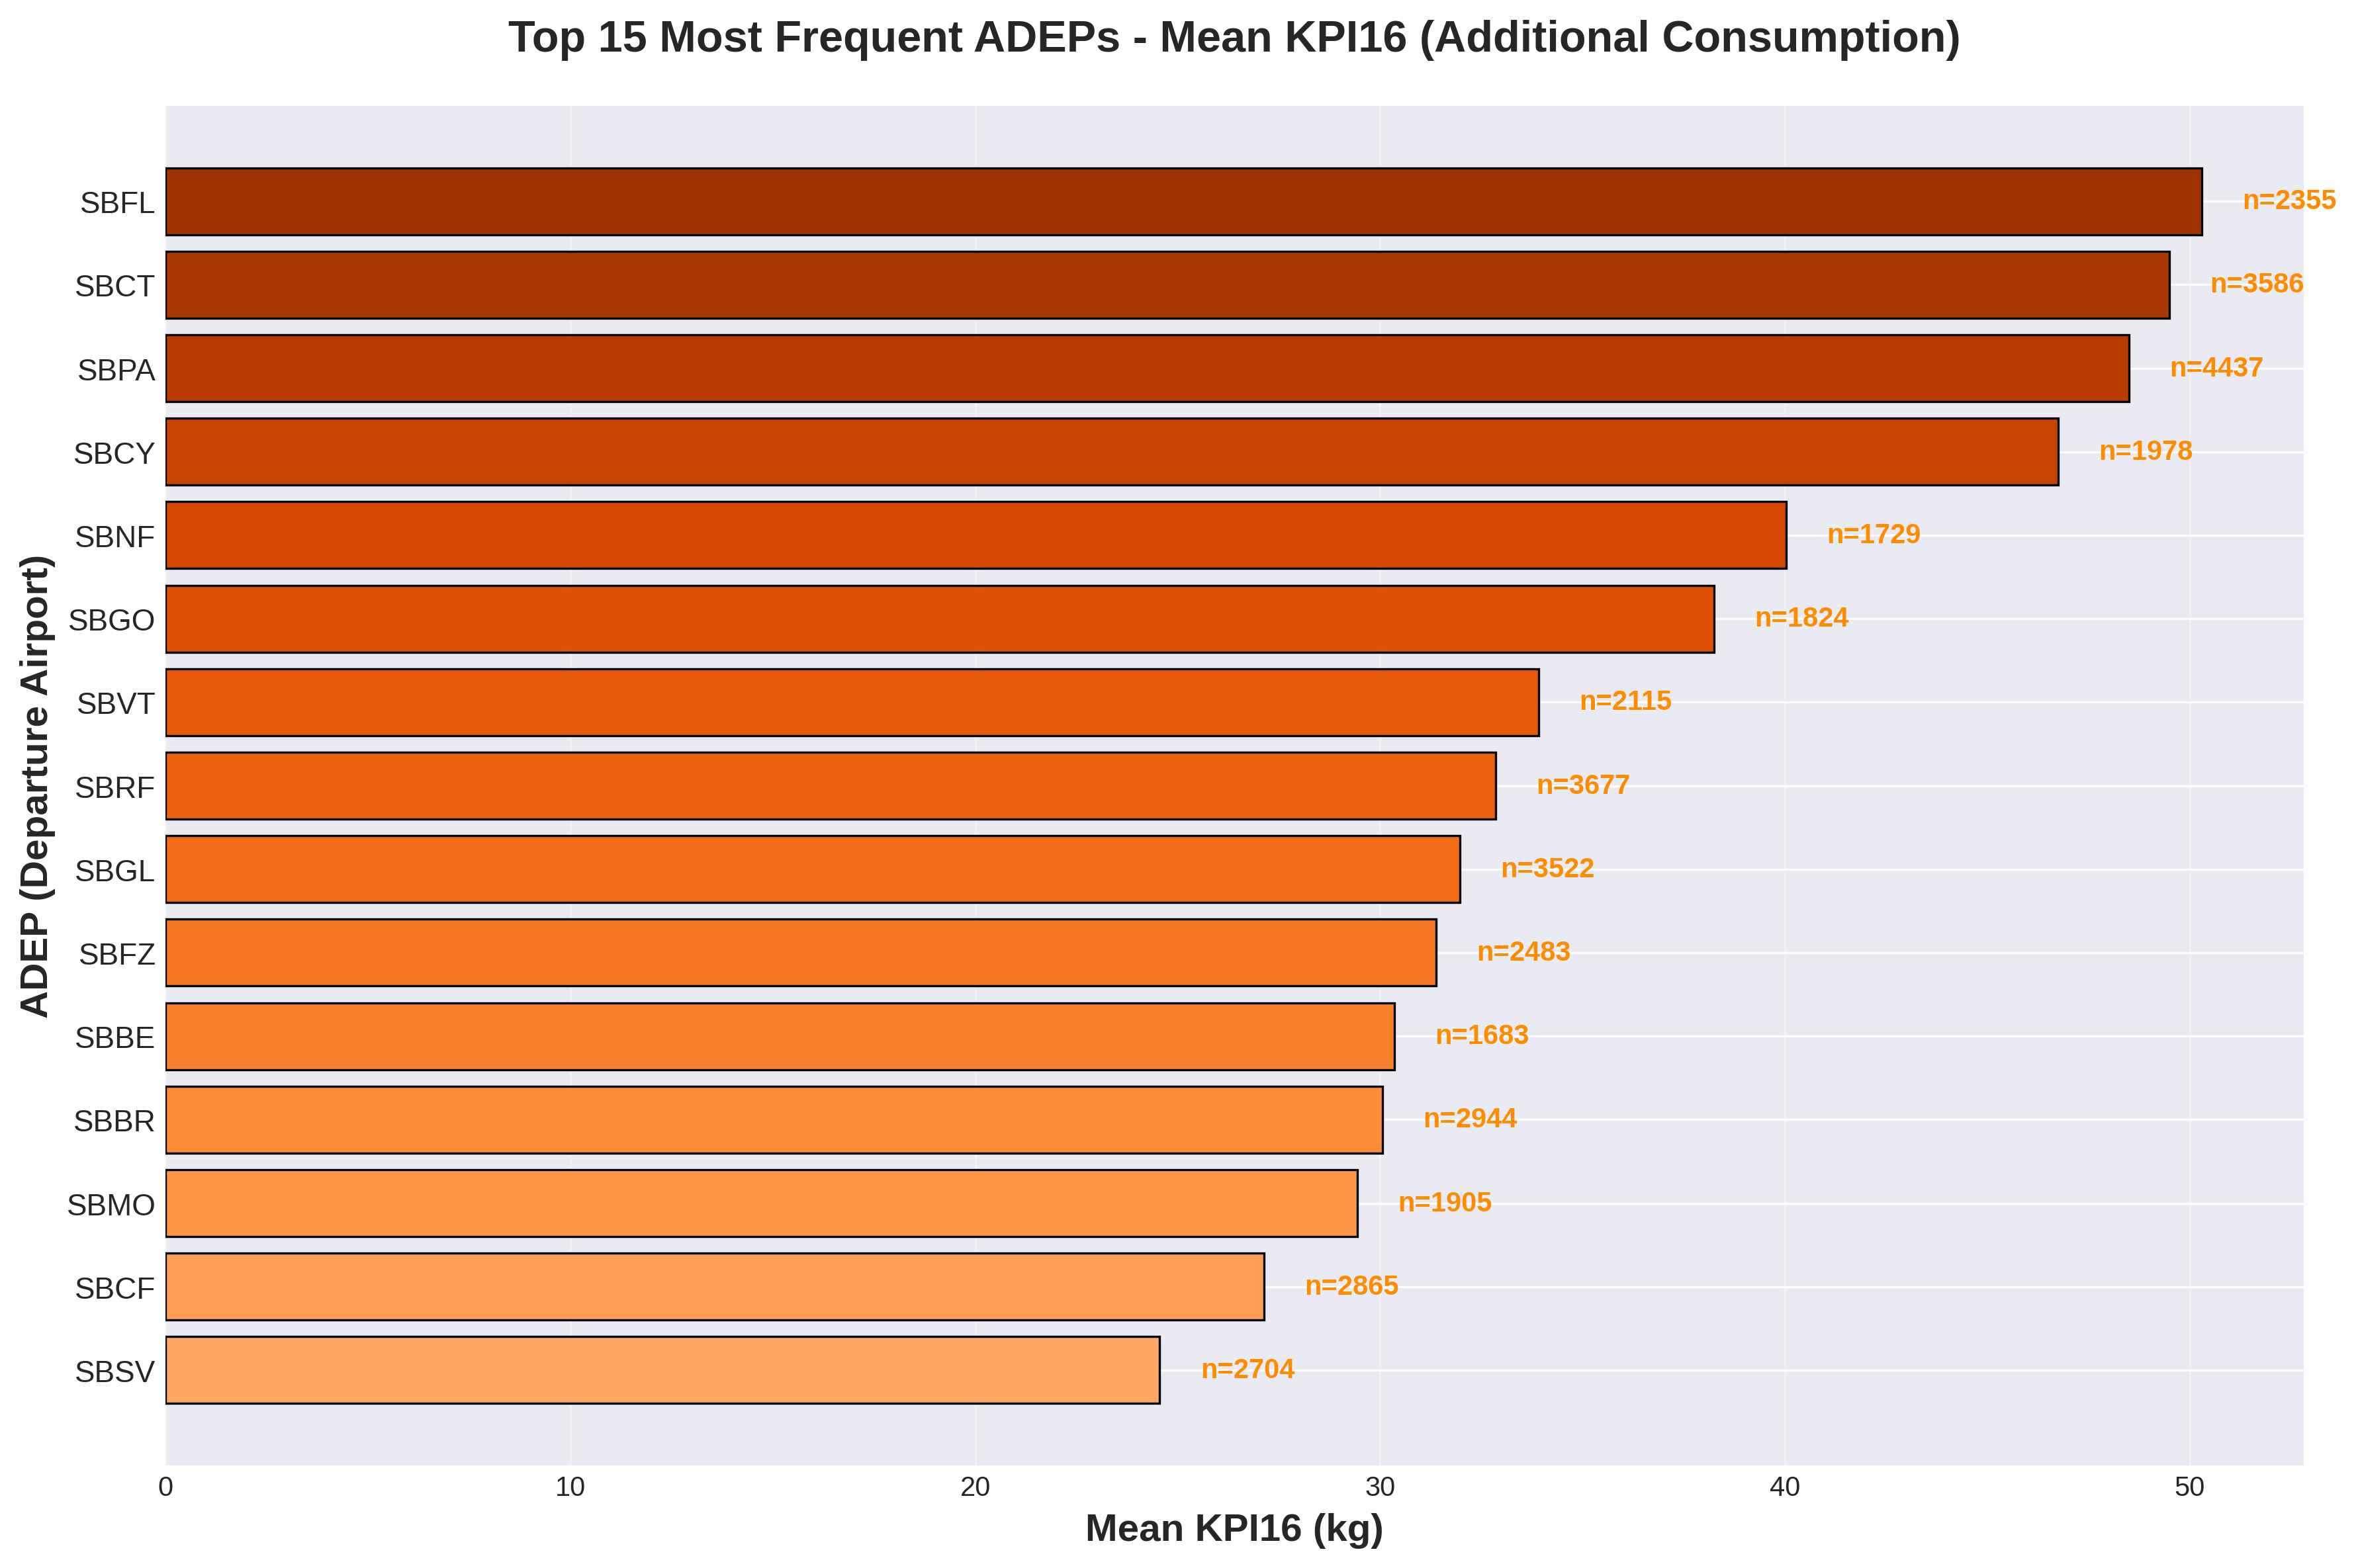
\includegraphics[width=1\linewidth]{images/adep_kpi16.png}
    \caption{Average additional fuel consumption (KPI16) by Departure Airport (ADEP).}
    \label{fig:adep-kpi16}
\end{figure}

\subsubsection{Impact of TMA Entry Sector on Efficiency}
To further investigate the geographical bottlenecks, the TMA was divided into entry sectors of 60-degree increments based on the aircraft's bearing upon crossing the terminal cylinder (excluding sector 120.0 due to insufficient sample size). As demonstrated in Figure \ref{fig:setor-kpi16}, flights entering through Sector 180.0 and Sector 300.0 demand the highest additional fuel consumption.

This pattern suggests that flights entering through these sectors may be associated with operational conditions that result in higher additional fuel consumption.

\begin{figure}[htbp]
    \centering
    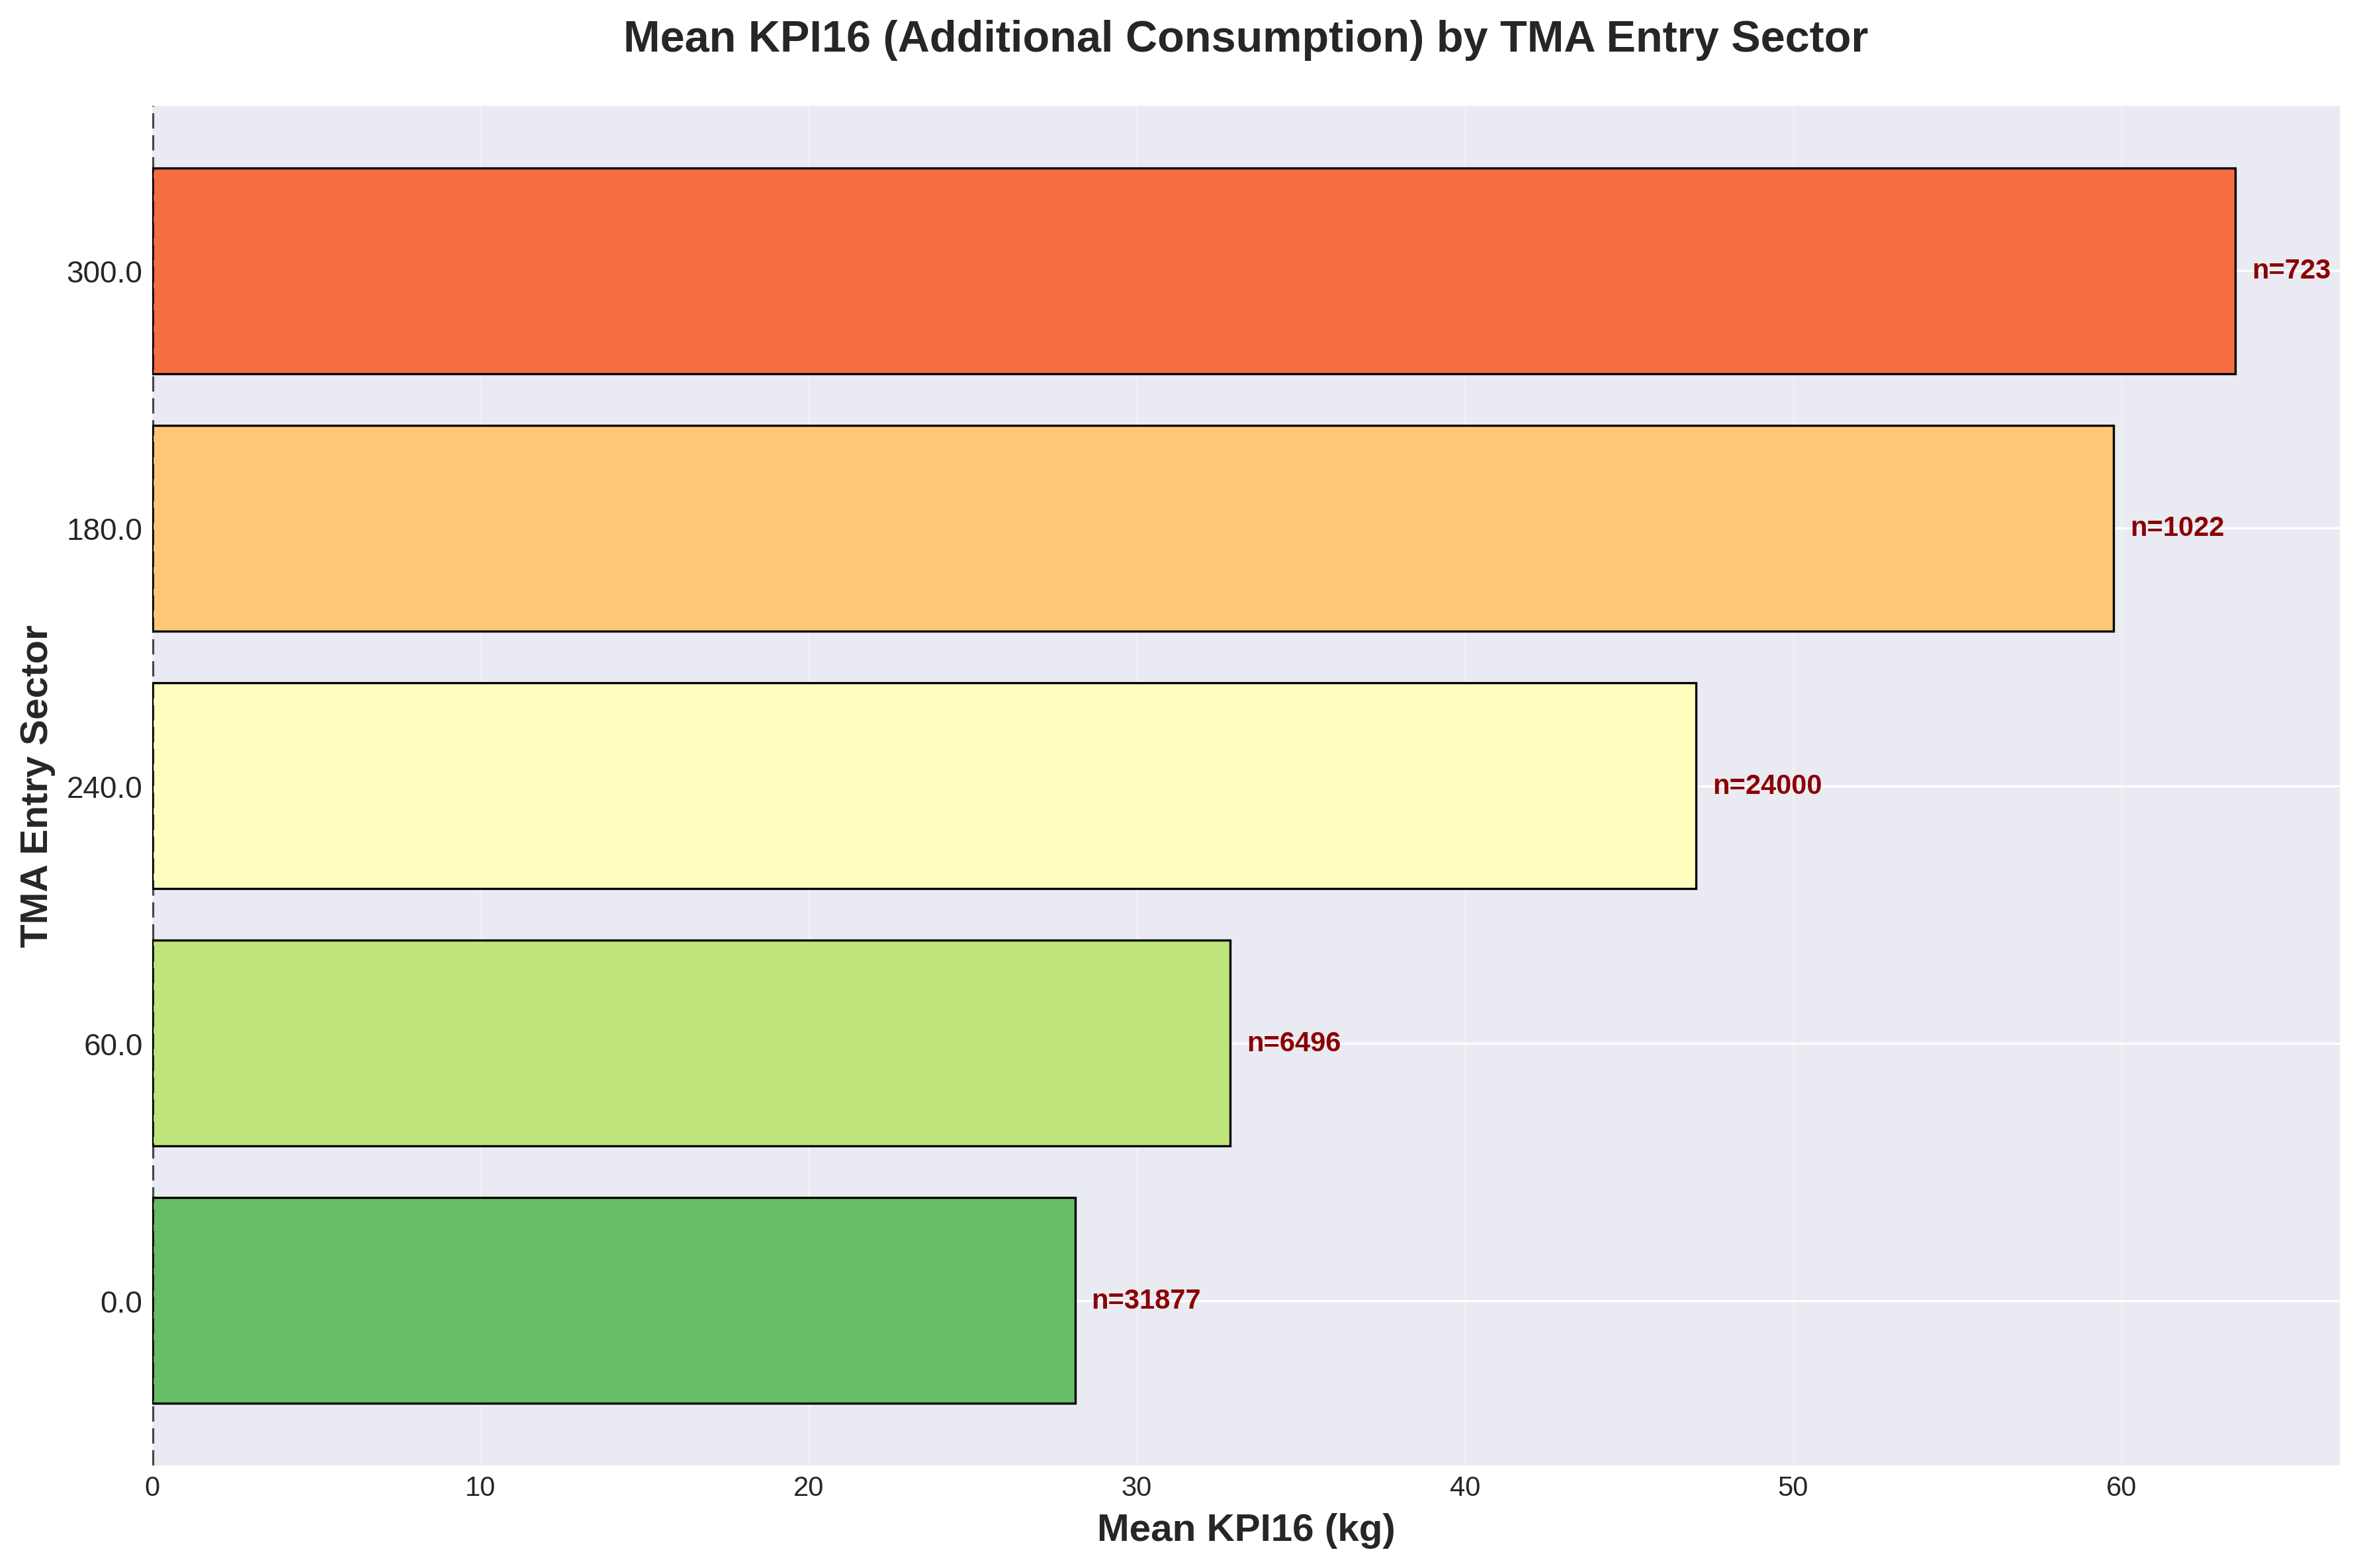
\includegraphics[width=1\linewidth]{images/setor_kpi16.png}
    \caption{Mean KPI16 (Additional Consumption) distributed by TMA Entry Sector.}
    \label{fig:setor-kpi16}
\end{figure}

\subsubsection{Interaction Between Entry Sectors and Origin Airports}
A more granular analysis combining both origin airports and entry sectors offers additional insight into factors that may contribute to the aforementioned inefficiencies. Figure \ref{fig:setor-adep-kpi16} details the most frequent ADEPs for the most penalizing sectors. Sector 180.0 is predominantly associated with flights from Southern capitals (Florianópolis, Porto Alegre, and Curitiba), while Sector 300.0 handles traffic from Goiânia, Uberlândia, and Manaus. The elevated additional fuel consumption observed in these sectors suggests that flights originating from these locations may be subject to more complex operational conditions within the TMA. One possible explanation is the convergence of multiple traffic flows into the same entry sectors, potentially increasing the complexity of arrival management and contributing to greater operational delays.

\begin{figure}[htbp]
    \centering
    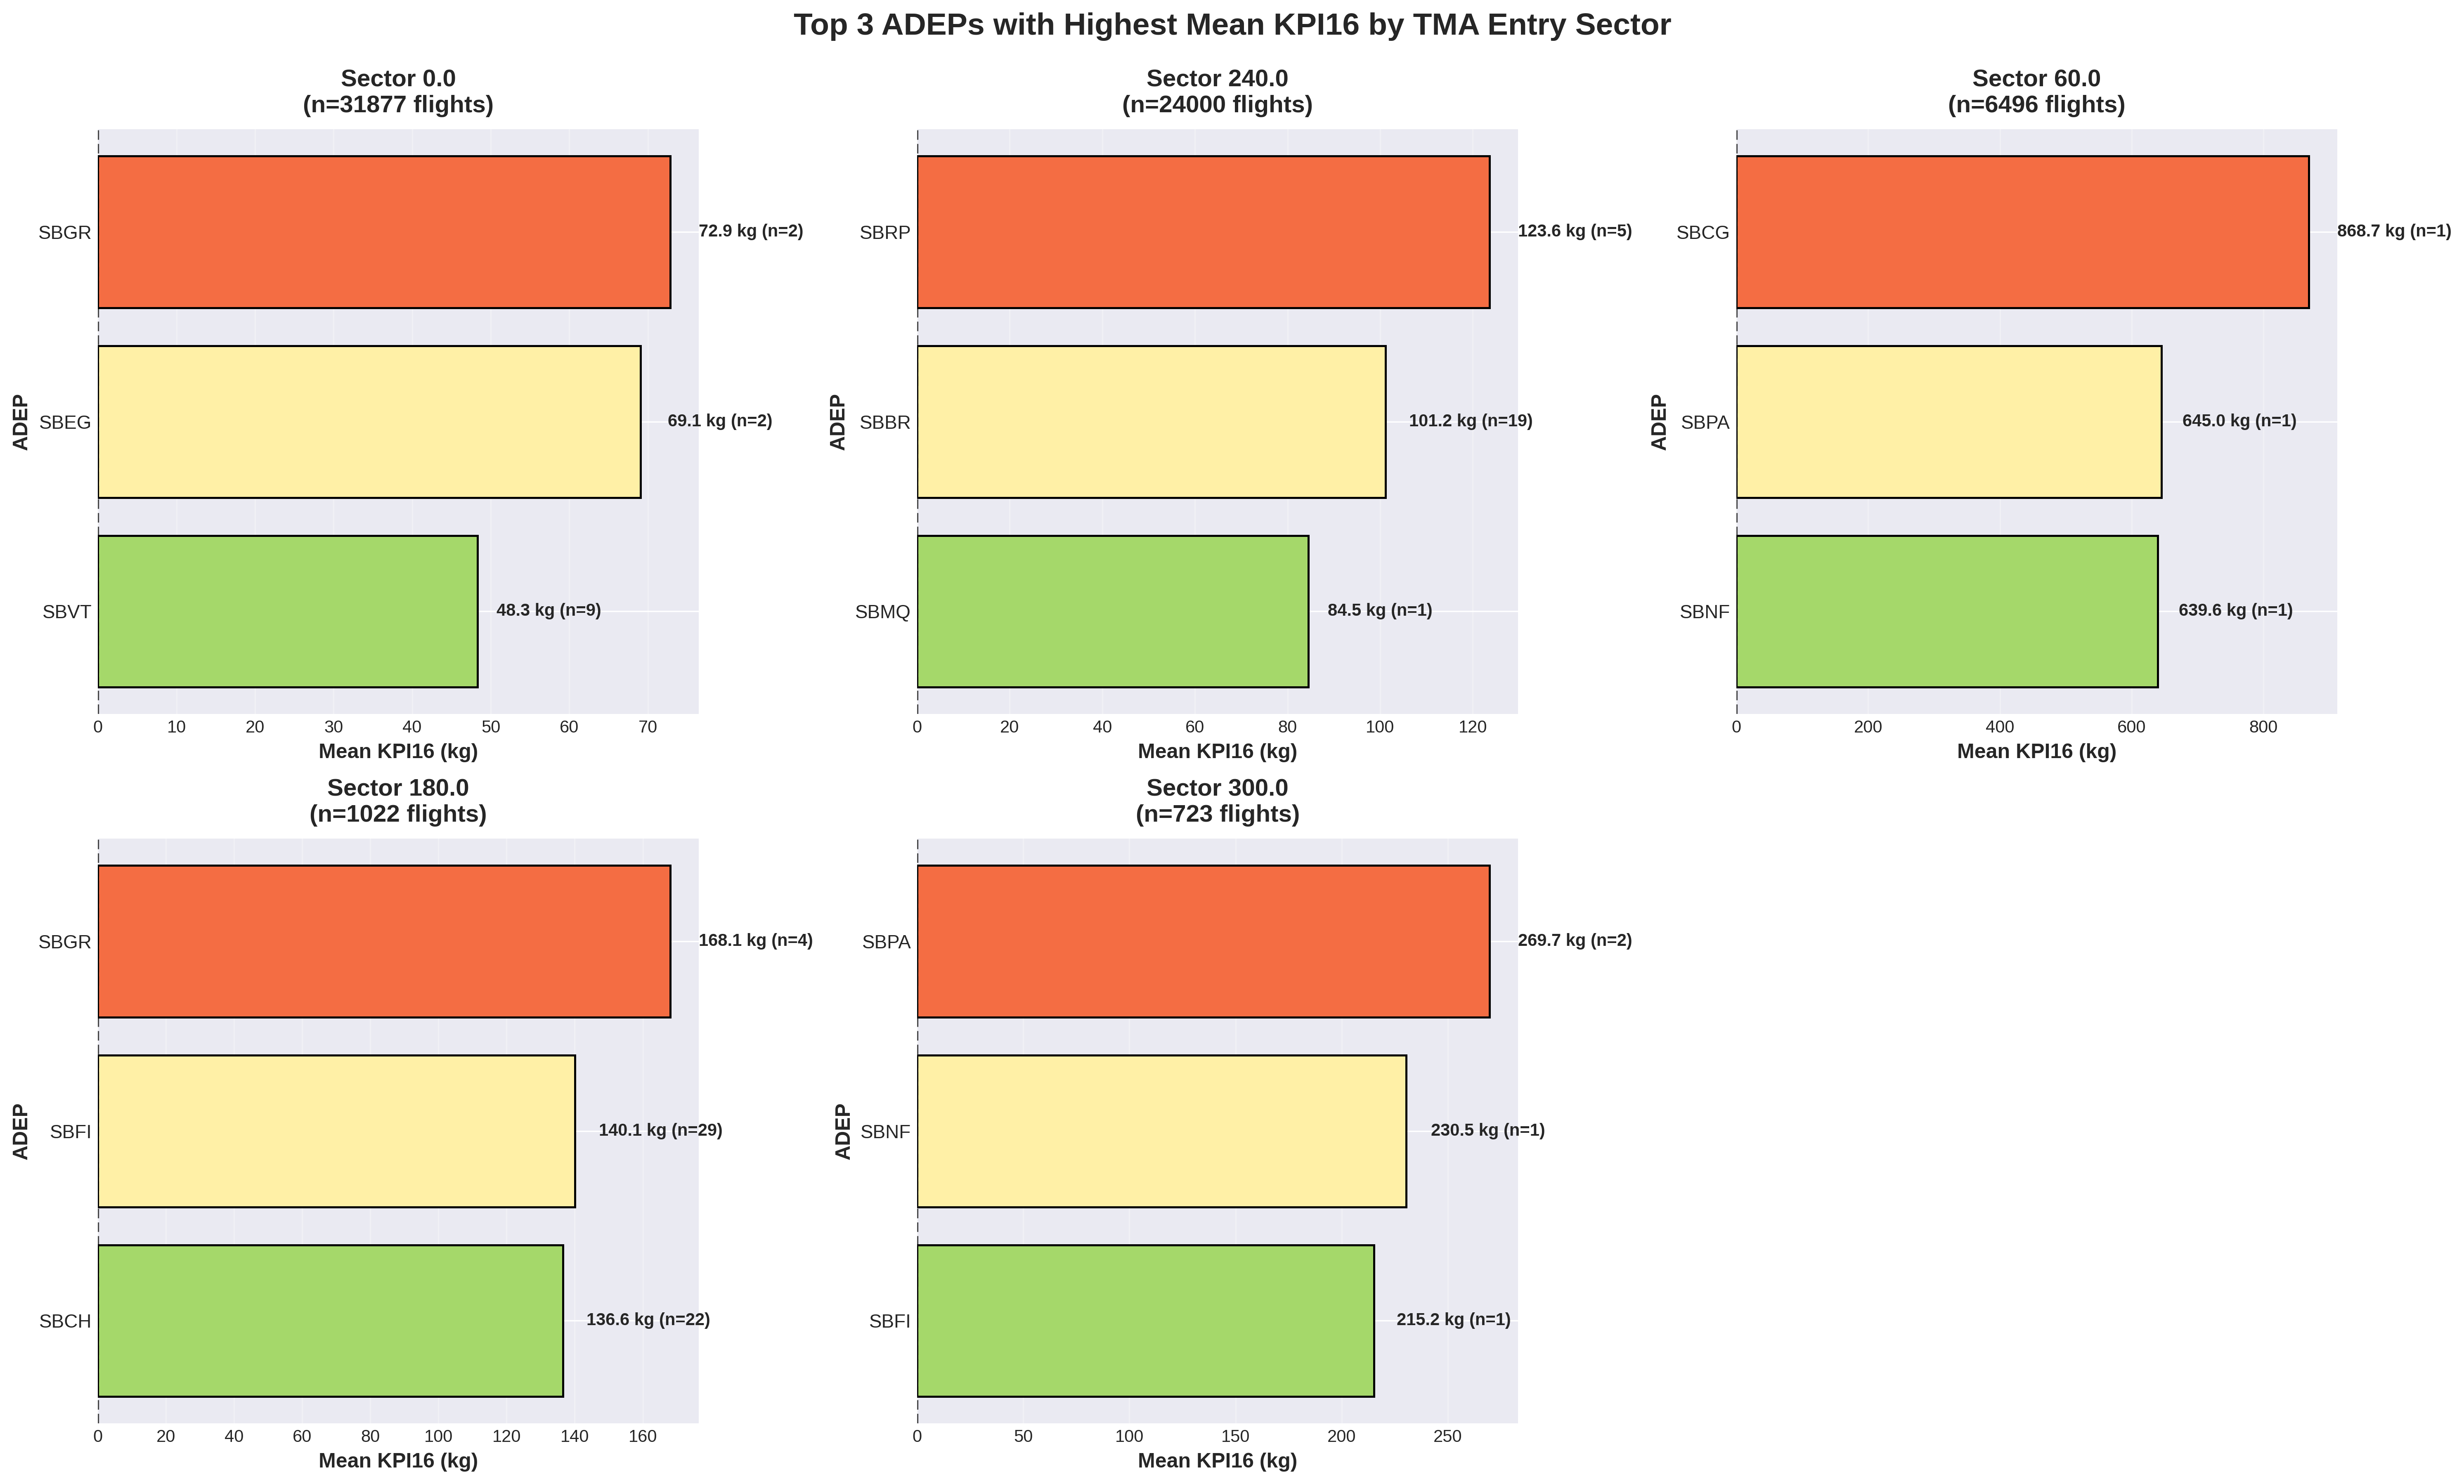
\includegraphics[width=1\linewidth]{images/setor_adep_kpi16.png}
    \caption{Top ADEPs contributing to high KPI16, grouped by TMA Entry Sector.}
    \label{fig:setor-adep-kpi16}
\end{figure}

To further support this observation, Figure \ref{fig:common-adep-sector} presents the share of total entries into each TMA entry sector attributed to the most frequent ADEPs. Notably, SBPA, SBCT, and SBFL together account for a dominant proportion of traffic entering through Sector 180, constituting evidence of traffic concentration rather than a confirmed causal mechanism. This concentration pattern may contribute to increased arrival management complexity, particularly when these flows overlap during peak periods.

\begin{figure}[htbp]
    \centering
    \includesvg[width=1\linewidth]{images/common_adep_sector}
    \caption{Share of total entries into each TMA entry sector by most frequent ADEPs, highlighting the dominant contribution of SBPA, SBCT, and SBFL to Sector 180 traffic volume.}
    \label{fig:common-adep-sector}
\end{figure}

\subsubsection{Hourly Traffic Variations and Congestion Cascading}
Air traffic operates in waves, and the time of arrival heavily dictates the level of congestion encountered. Figure \ref{fig:hora-adep} groups the performance of the three most impactful ADEPs across the six busiest hours of the day. During peak periods, flights originating from SBPA, SBCT, and SBFL appear to concentrate in Sector 180, which may increase the operational complexity of the traffic and contribute to the higher KPI16 values observed in the flow. Consequently, flights from Florianópolis (SBFL) sharing the same entry sector are often associated with elevated fuel penalties, suggesting a cascading effect on overall performance.

\begin{figure}[htbp]
    \centering
    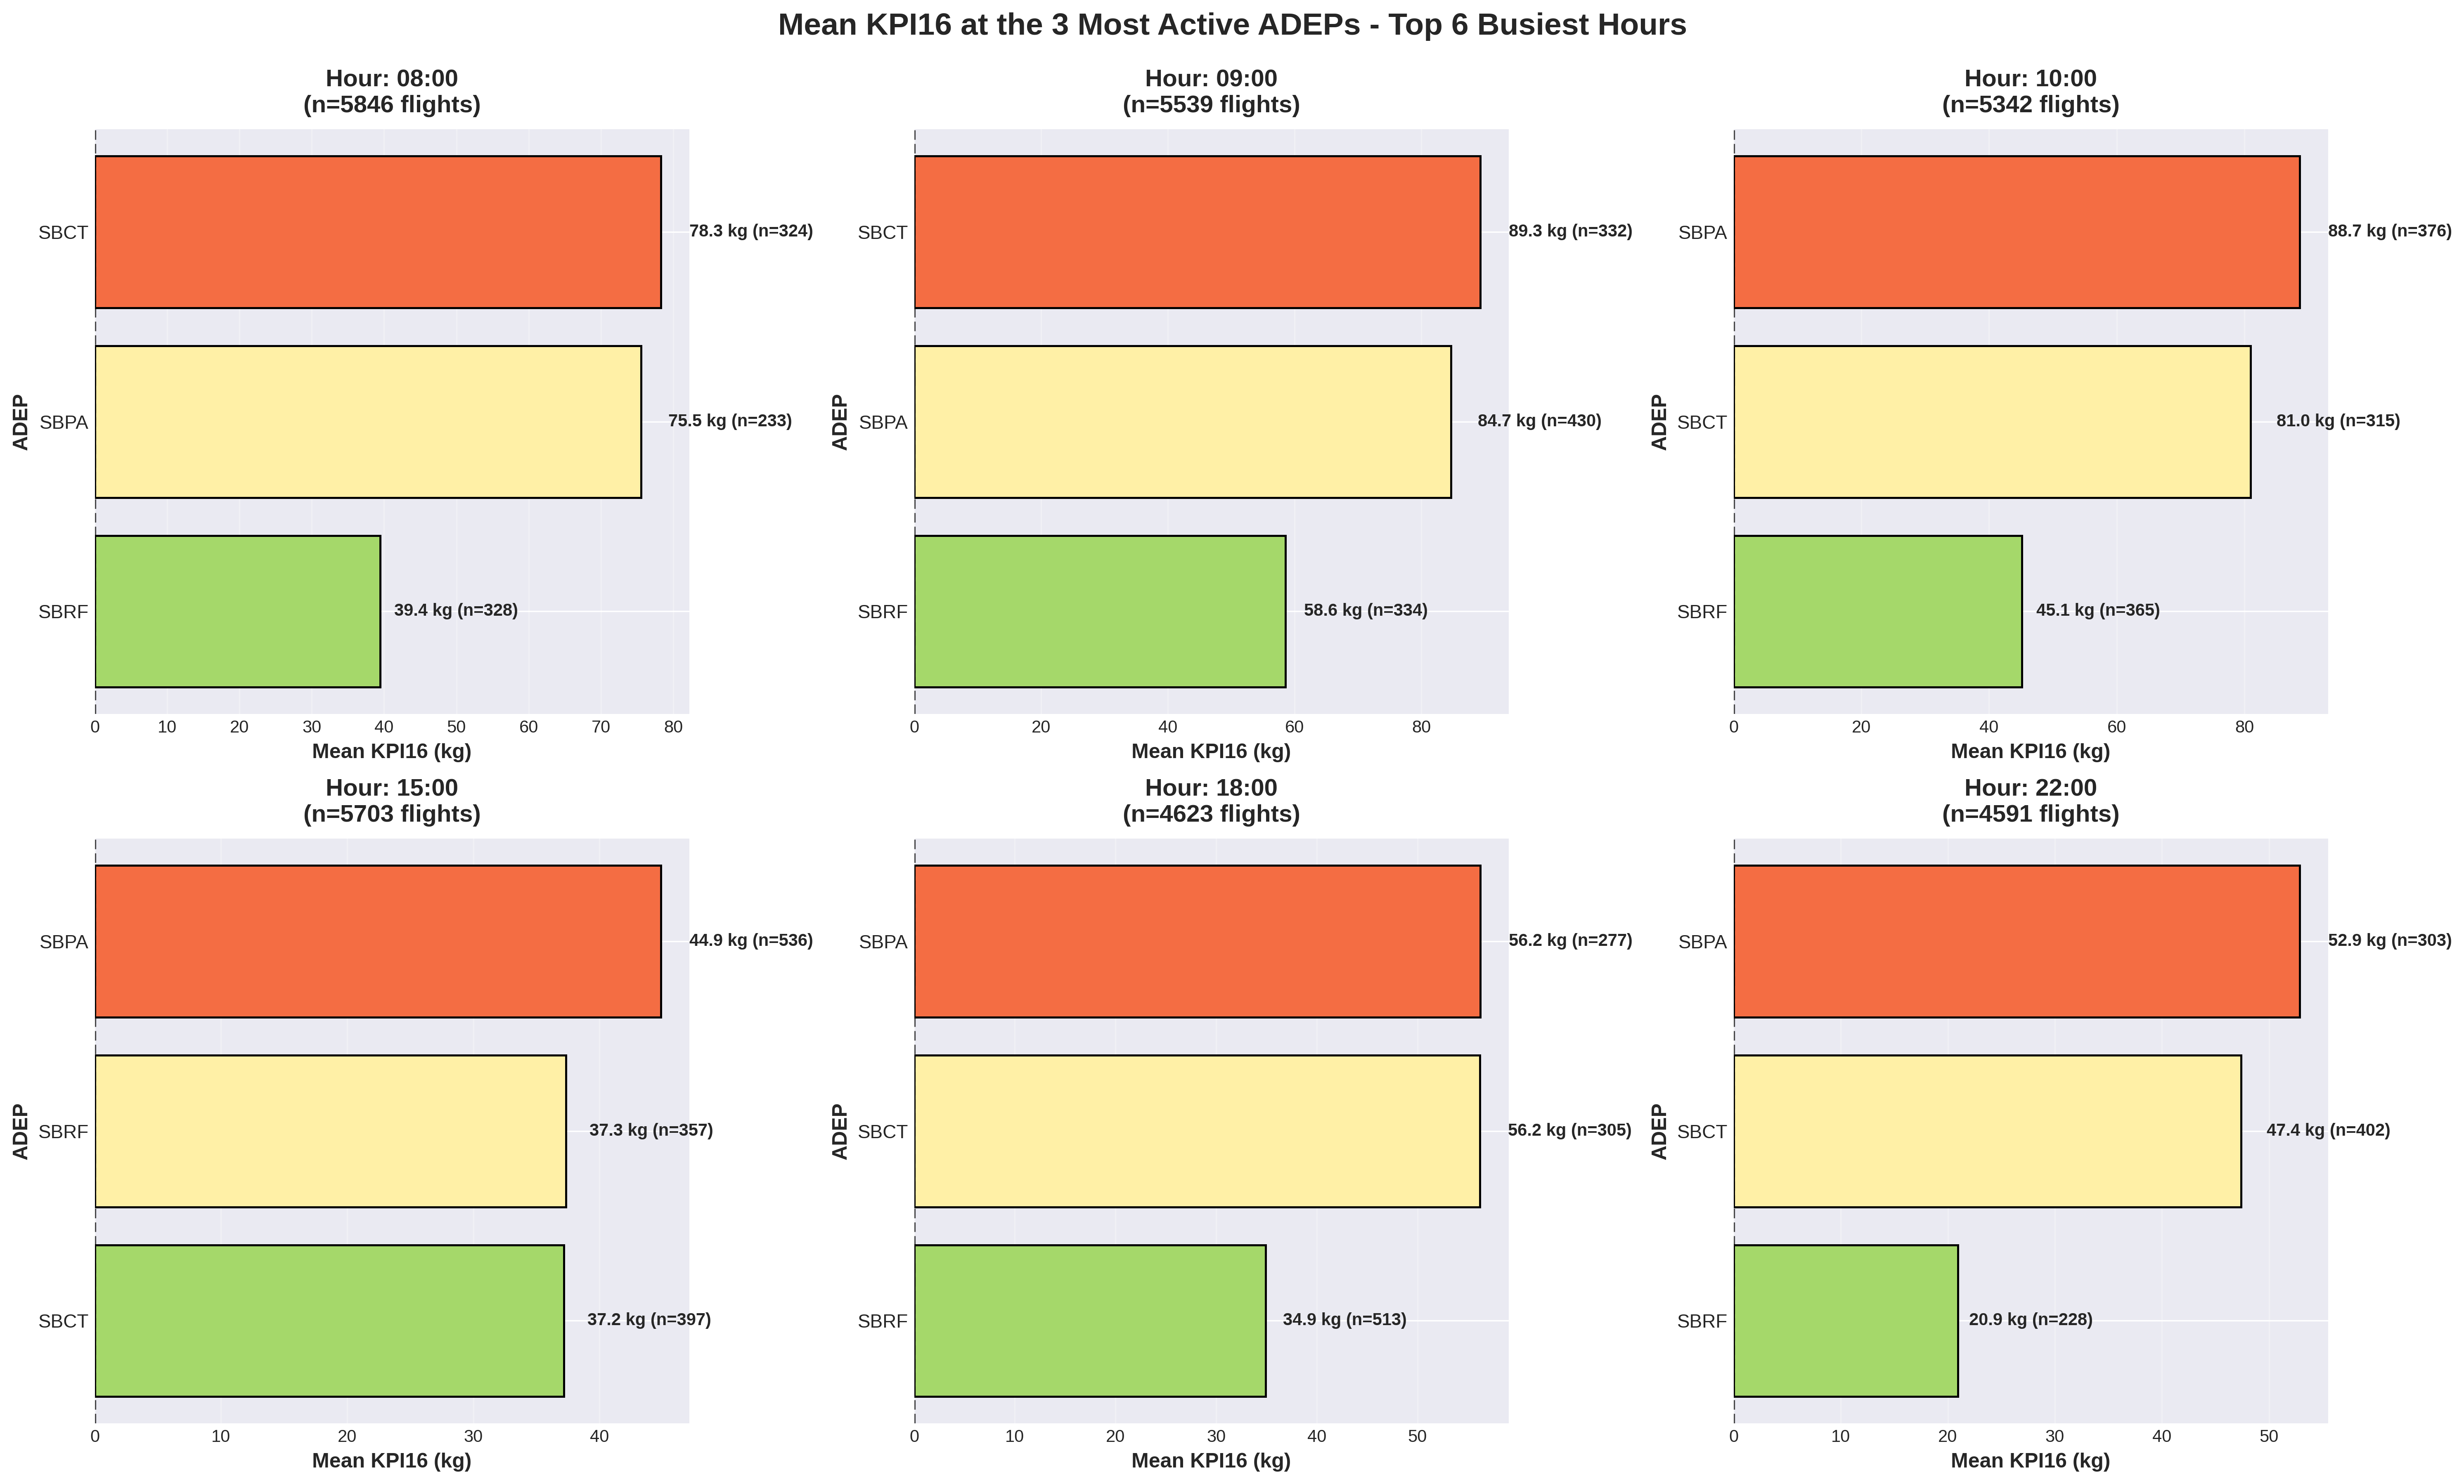
\includegraphics[width=1\linewidth]{images/hora_adep.png}
    \caption{Mean KPI16 for the three most active ADEPs during the top six busiest landing hours.}
    \label{fig:hora-adep}
\end{figure}

\subsection{Machine Learning Approach}
To evaluate the predictability of the additional fuel consumption ($kpi16$) given the operational, spatial, and meteorological conditions prior to or at the exact moment the aircraft enters the Terminal Control Area (TMA), we formulated the problem as a supervised machine learning regression task.

A rigorous pipeline was established to prevent data leakage: features that could only be observed after the flight's landing (e.g., total transit time, actual fuel consumed) were strictly excluded from the predictive models. This ensures the integrity of time-series estimations, a common pitfall observed in environmental and operational monitoring tasks \cite{dataleakage}. The final set of explanatory variables included both numerical features (e.g., number of concurrent aircraft in the TMA, predicted transit time based on a rolling window, visibility, and cloud ceiling) and categorical features (e.g., origin airport, aircraft type, entry sector, validated runway, month, hour, and day of the week).

Missing values in the cloud ceiling variable were imputed with a constant high value (10,000 ft) assuming clear sky conditions, while other numerical variables were imputed using their respective medians. For the baseline linear model, categorical features were encoded using One-Hot Encoding and numerical features were normalized using Standard Scaling. For a fair and direct comparison, this exact same pre-processed dataset was utilized across all evaluated algorithms, employing a randomized train-test split with an 80/20 ratio (51,295 records for training and 12,824 for testing).

We benchmarked six distinct machine learning algorithms to map the complex, non-linear relationships of airspace congestion to fuel consumption.

\subsubsection{Linear Regression (Baseline)}
To establish a performance baseline, an Ordinary Least Squares (OLS) Linear Regression \cite{hastie2009elements} was trained. While highly interpretable and computationally efficient, linear regression assumes a linear relationship between the predictors and the target variable. In highly complex environments like air traffic management, this model serves as a simple and interpretable benchmark.

\subsubsection{Random Forest Regressor}
Random Forest \cite{breiman2001random} is a robust ensemble learning method that operates by constructing a multitude of decision trees during training and outputting the average prediction of the individual trees. It uses a bagging (bootstrap aggregating) technique to reduce variance and avoid overfitting. We configured the model with 100 estimators and a maximum depth of 15 to balance model complexity and generalization capacity.

\subsubsection{Gradient Boosting Regressor}
Gradient Boosting \cite{friedman2001greedy} is a sequential ensemble technique where each new decision tree is trained to correct the residual errors made by the previous trees. It is highly effective for tabular data with heterogeneous features. The Scikit-Learn implementation of the Gradient Boosting Regressor was trained using 100 estimators, a learning rate of 0.1, and a maximum tree depth of 5.

\subsubsection{XGBoost}
Extreme Gradient Boosting (XGBoost) \cite{chen2016xgboost} was selected due to its proven performance on structured tabular datasets and its ability to model complex nonlinear interactions between traffic, operational, and meteorological variables. It incorporates advanced regularization (L1 and L2) to prevent overfitting. For our tabular dataset, we utilized the histogram-based tree method (\texttt{tree\_method='hist'}), which significantly speeds up the training process. The model was parametrized identically to the standard Gradient Boosting (100 estimators, learning rate of 0.1, maximum depth of 5).

\subsubsection{LightGBM}
Light Gradient Boosting Machine (LightGBM) \cite{ke2017lightgbm}, developed by Microsoft, is a gradient boosting framework that uses tree-based learning algorithms. It is designed for distributed and efficient training, notably using a leaf-wise (rather than level-wise) tree growth strategy. This allows for faster convergence and lower memory usage. We trained the LightGBM model with 100 estimators, a learning rate of 0.1, and a maximum depth of 5.

\subsubsection{CatBoost}
Categorical Boosting (CatBoost) \cite{prokhorenkova2018catboost}, developed by Yandex, is an algorithm that natively handles categorical variables without the need for extensive pre-processing (like One-Hot Encoding). It uses oblivious decision trees, which decreases scoring time and avoids overfitting. Although CatBoost is capable of processing raw categorical data, we trained it on our pre-processed dataset for a strict one-to-one benchmark. The model was configured with 100 iterations, a learning rate of 0.1, and a depth of 5.
